
\chapter{Implementierung}

In diesem Kapitel wird auf Besonderheiten bei der Implementierung eingegangen.


%Weitestgehend wie in \autoref{draft:architecture}, aber Futures, tokio, Queues

\todo{diagramm message decode steps}

\todo{proxy communication}

\section{Bindgen für ASN}

\label{impl:issue:ffi}
\todo{schnell problem: kein asn->rs compiler, c bindings aufwending -> autogen via bindgen}

\todo{link issues fixed in commit d5d694c}

\todo{impl Drop / free structs, important but do not overengineer}


\subsection{Continuous Integration mittels Jenkins}

Mittels der Continuous Integration Software Jenkins wird die Rust-Implementation nach jeder Aktualisierung der Quellcode-Repository gebaut.
In einem Jenkinsfile ist hierzu die folgende Pipeline definiert:

\begin{figure}[H]
	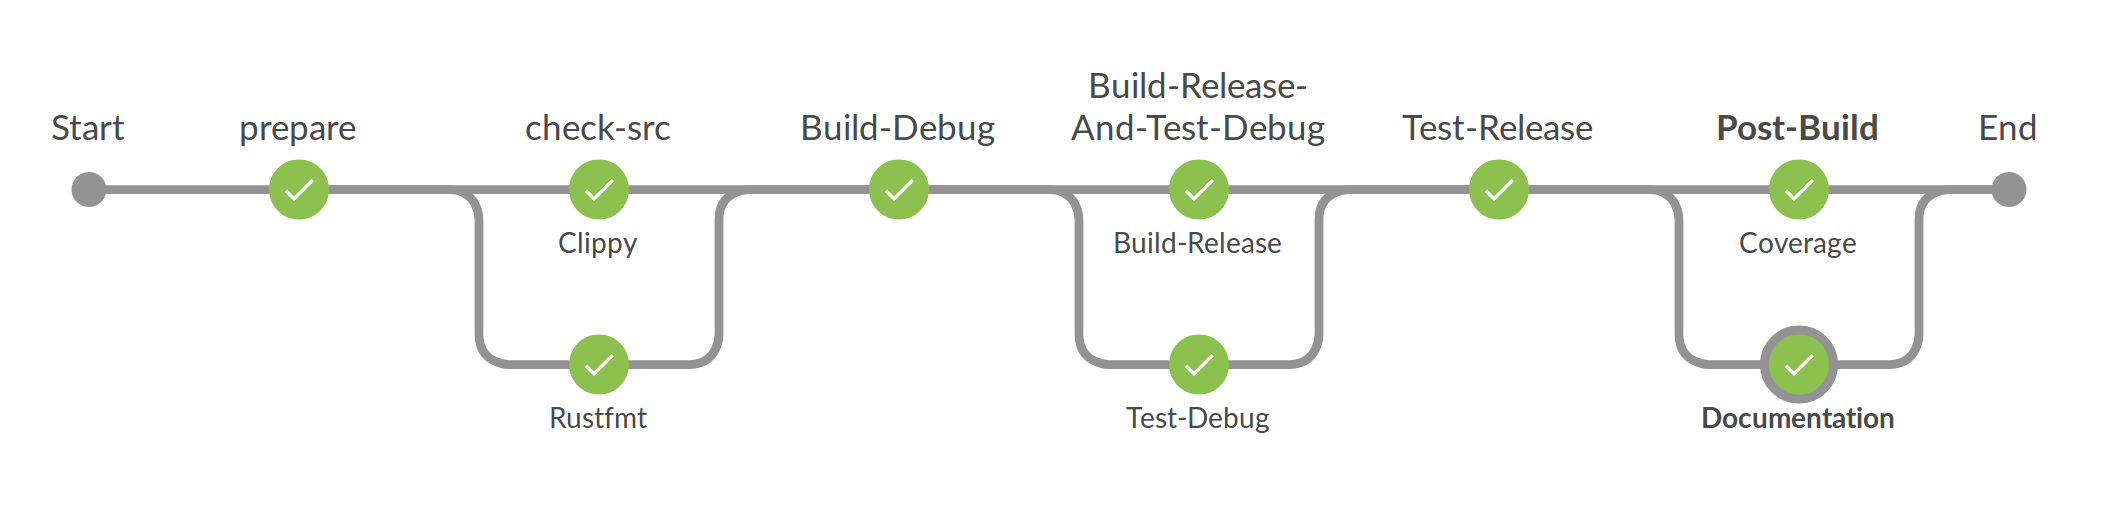
\includegraphics[width=\textwidth]{images/jenkins_pipeline_graph.png}
	\caption{Jenkins Pipeline Graph}
	\label{impl:jenkins:pipeline:graph}
\end{figure}

Im folgenden sind die einzelnen Schritte genauer erklärt.


\subsubsection{Schritt \enquote{prepare}}
In diesem Schritt wird überprüft, ob die richtige Version von Rust installiert ist.
Sowohl der Rust Compiler als auch Abhängigkeiten wie Cargo, Clippy oder Tarpaulin werden falls nötig  in diesem Schritt nachinstalliert und aktualisiert.

\subsubsection{Schritt \enquote{check-src}}
Hier wird der Quellcode auf einen schlechtem Programmierstil oder schlechte Programmierpraktiken durch Clippy und auf eine nicht standardkonforme Formatierung überprüft.
Ein erkannter Mangel resultiert in einem abgebrochenem Bauversuch und einem entsprechendem roten Icon auf der Projektseite auf Jenkins.
Ein Quellcode, der diese Qualitätsstandards nicht erfüllt, wird somit schnellstmöglich abgelehnt.

\subsubsection{Schritt \enquote{Build-Debug}}
In diesem Schritt wird das Projekt und Abhängigkeiten im Debug-Modus kompiliert.
In einem Debug-Modus werden nahezu keine Optimierungen durchgeführt, weswegen die Ausführgeschwindigkeit meist mangelhaft ist.
Im falle eines Fehlers in einem Unit-Test, können in aus einem Debug-Artefakt jedoch nützlich Informationen gewonnen werden.

\subsubsection{Schritt \enquote{Build-Release-And-Test-Debug}}
Wie der Name bereits vermuten lässt, wird in diesem Schritt das Projekt im Release-Modus übersetzt.
Gleichzeitig wird das zuvor erstellte Debug-Artefakt auf Fehler überprüft, indem Unit-Tests ausgeführt werden.
Ein Release-Artefakt ist stark optimiert und ist für den Produktivbetrieb gedacht.

\subsubsection{Schritt \enquote{Test-Release}}
In diesem Schritt wird das Release-Artefakt mittels Unit-Tests auf Fehler überprüft.
Hierdurch soll sichergestellt werden, dass kein Fehler durch Optimierungen des Compilers aufgedeckt oder verursacht wurden.
\todo{.} Auch soll kein Artefakt für den Produktivbetrieb empfohlen werden, das nicht auf Fehler überprüft wurde.

\subsubsection{Schritt \enquote{Post-Build}}
Dieser Schritt dient zur Zusammenstellung der Testabdeckung der Unit-Tests und der automatisierten  Erstellung der Dokumentation.

\subsubsection{Ergebnis des erfolgreichen Durchlaufs}
Jede Aktualisierung der Quellcoderepository resultiert bei erfolgreicher Kompilation und durchlaufen der Tests in den folgenden Artefakten:
\begin{itemize}
	\item \textbf{Debug-Artefakt}: Kompilation für eine manuelle Fehlersuche mit vielen auf den Quellcode bezogenen Symbolen und ohne Optimierungen durch den Compiler
	\item \textbf{Release-Artefakt}: Kompilat mit Optimierungen für den Produktivbetrieb
	\item \textbf{\todo{Unit-Test-Abdeckungsbericht}}: Bericht über wie viele Zeilen, Dateien, Klassen und Verzweigungen durch die Unit-Tests getestet wurden.
	\item \textbf{Dokumentation}: \todo{.}
\end{itemize}

Für jeden erfolgreichen Bauversuch, werden die erhobenen Informationen in die folgenden Graphen auf der Projektseite auf Jenkins übernommen:

\begin{figure}[H]
	\centering
	\begin{subfigure}{.5\textwidth}
		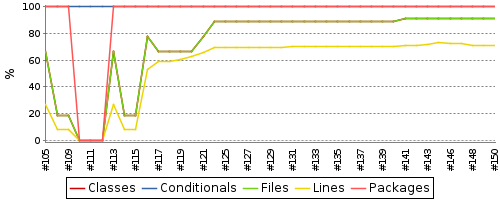
\includegraphics[width=\textwidth]{images/jenkins_coverage_graph.png}
		\caption{Jenkins Coverage Graph}
		\label{impl:jenkins:coverage:graph}
	\end{subfigure}%
	\begin{subfigure}{.5\textwidth}
		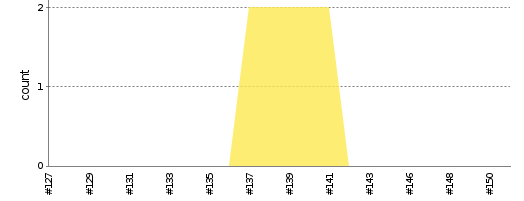
\includegraphics[width=\textwidth]{images/jenkins_warnings_graph.png}
		\caption{Jenkins Warnings Graph}
		\label{impl:jenkins:warnings:graph}
	\end{subfigure}
\end{figure}

\autoref{impl:jenkins:coverage:graph} zeigt die Testabdeckung seit Aufzeichnungsbeginn.
Die frühen und starken Schwankungen resultieren aus Testdurchläufen bei der Einrichtung des Graphen.
\autoref{impl:jenkins:warnings:graph} zeigt Warnungen die der sehr \todo{pingelige} Rust Compiler für die verschiedenen Builds ausgegeben hat.

Die Graphen starten bei unterschiedlichen Baunummern, da sie nacheinander eingerichtet wurden.

\todo{bzgl coverage viele tests für encodieren / decodieren, server instanz nicht getestet weil nur mit tokio verdrahtet... schwierig zu testen}

\section{...}

\todo{tdd schwierig weil viel integration mit framework / async, schnell wird daraus integrationstest(?, unerwünscht)}

\todo{rust-clippy: https://github.com/rust-lang-nursery/rust-clippy}


\section{Strategien für Performance}

\todo{\enquote{bypass} for algorithm->>many vehicles}





\todo{diagramm: jede future ein eigenes "paket", queues dazwischen für kommunikation}

\todo{catch panic? mention how in \autoref{rust:no_null}}

\todo{SRP, impl Object separat from impl CommandProcessor for Object, testability?}

\subsection{Tokio}

	\subsection{Generalisierung mittels Aufzählung für nicht erweiterbare Anzahl von Elementen}
	
	\subsection{libmessages make unsafe libmessages-sys safe}
	
	\subsection{Vorgehen, bindgen tests, C/unsafe/wrapper -> nach sicher ->  architektur entwickeln}
	

	
	\subsection{Unerwartete Schwierigkeiten}
	
	\todo{Trailing zeroes issue, commit a02496d + tagged, libmessages/src/asn.rs:17 bzw :31 bzw :32 Ok((result.encoded as usize + 7) / 8}
	
	\todo{unterschiedlicher Heap libc / rust}
	
	\todo{jenkins clippy nightly often broken}
	
	
	\subsection{--help}

\todo{bei der entwicklung nie segfault/deadlock gehabt, nur einmal heap problem wegen libc}


\section{Valgrind: Race Conditions all over the place}